% !TEX root = main.tex
\chapter{Analysis}
\label{analysis}

\section{Computation Preface}

For the following analyses, the algorithm was run on a 2018 Dell XPS 15 laptop with an Intel quad-core i7-7700HQ CPU clocked at 2.8GHz with 16GB of ram. The implementation was in Python utilizing CVXpy configured to use the ECOS solver by EmboTech \cite{domahidi2013ecos}. ECOS is an Mehrotra predictor corrector interior-point method (IPM) solver for second-order cone programs (SOCP) designed specifically for embedded applications.

It should be understood that this Python implementation of this is not optimized to run quickly on embedded platforms and should not be held as a benchmark. These algorithms are amenable for online implementation and should be written in C/C++ ideally with customized solvers that can take advantage of the problem structure. One can reach excellent cycle speeds for these algorithms as evidence by \cite{szmuk2019successive}. The performance and computational information presented in this section was performed with the baseline problem outlined in Table \ref{table:tableplanar}.

Additionally, it should be understood that all runs listed were initialized with a dynamically infeasible and linearly-spanned trajectory as discussed earlier. These are suboptimal with respect to performance and will required larger numbers of iterations compared to a good guess. One could easily improve this with an LQR run or another dynamically-motivated trajectory generation algorithm. This would significantly decrease computation time for the SCvx algorithm.

\section{Temporal Node Count Variation}
Although the listed runtimes are larger than nominal for an implementation, for the aforementioned reasons, it important to study it's numerical behaviour. Table \ref{table:timingtable} shows the planar problem shown in \ref{table:tableplanar} being solved numerous times for the temporal node count quantity K for cases of $K = [10, \ 15, \ 20, \ 30, \ 40, \ 50]$. For trajectories with 10 state and control temporal nodes, the computer took an average of 1.771 seconds to compute. Figure \ref{fig:finaltimeplot} shows how the final time solution changes on the order of 100ms from a K=10 solution to a K=50 solution. Additionally, the final time difference between K=20 and K=50 is less than 100ms and shows that the latter is not necessarily better for the extra computation cost. Similarly in Figure \ref{fig:massdisperse}, where the key metric of remaining final mass is displayed with respect to K, it is shown that increasing the temporal resolution does not necessarily save much more fuel. The difference between a quick calculation and a more intensive one is on the order of hundreds of grams, effectively inconsequential.


\begin{table}[ht]
\caption{Computation Time (seconds)}
\centering 
\begin{tabular}{c c c c c} 
\hline\hline \\[0.5ex] 
K & Min & Max & Mean & Stdev \\ 
\hline \\
$10$    &$0.875 $   &$1.771 $  &$1.3023  $  &$0.29$   \\ 
$15$    &$1.331 $   &$2.713 $  &$2.2504  $  &$0.365$  \\ 
$20$    &$2.289$    &$2.986$   &$2.618  $   &$0.230$  \\ 
$30$    &$ 3.38 $   &$4.708 $  &$4.1419  $  &$0.363$  \\ 
$40$    &$4.587 $   &$5.499 $  &$4.9056  $  &$0.257$  \\ 
$50$    &$6.814 $   &$8.637 $  &$7.7515  $  &$0.688$  \\[1ex] 
\hline
\end{tabular}
\label{table:timingtable}
\end{table}

Figure \ref{fig:solvetimes} shows the results of Table \ref{table:timingtable} in a graphical form for multiple runs. For the same landing problem, it is shown that the convergence rate in Figure \ref{fig:iterations} of each of the resolution problems is effectively the same. For our K=10 case, a converged solution was extracted after the 13th successive iteration.


\begin{figure}[!htbp] 
\label{}
  \centering
  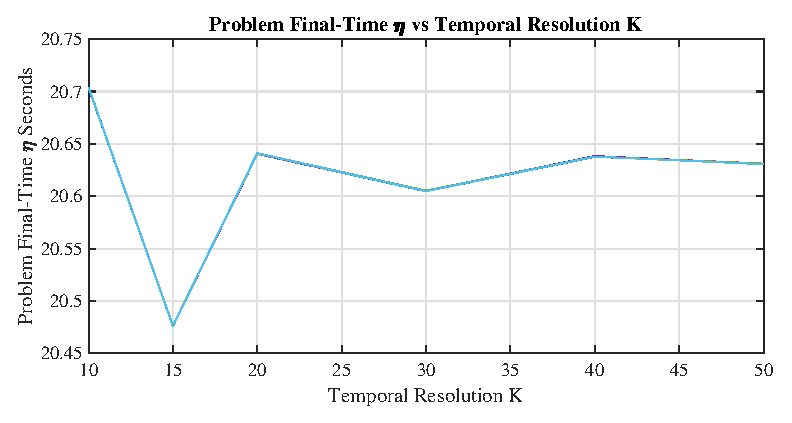
\includegraphics[width=\textwidth]{figs/etavsK.eps}
  \caption{Planar Guidance Problem: Final-Time $\eta$ versus Temporal Node Count K}
  \label{fig:finaltimeplot}
\end{figure}

\begin{figure}[!htbp] 
\label{}
  \centering
  \includegraphics[width=\textwidth]{figs/massvsK.eps}
  \caption{Planar Guidance Problem: Terminal Vehicle Mass versus K Node Count}
  \label{fig:massdisperse}
\end{figure}

\begin{figure}[!htbp] 
\label{}
  \centering
  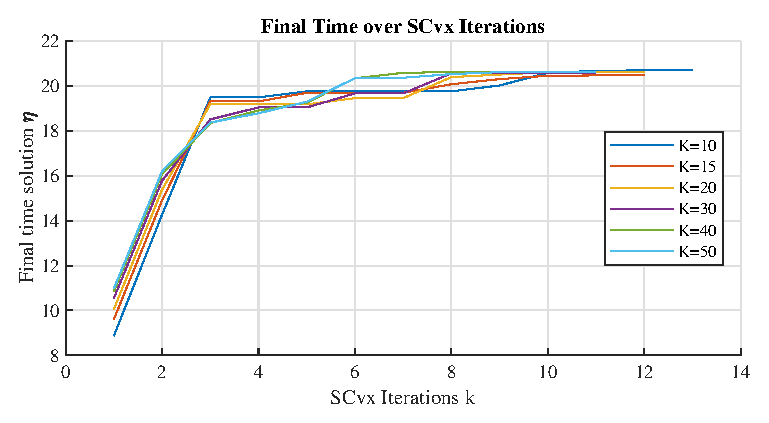
\includegraphics[width=\textwidth]{figs/iteratetiming.eps}
  \caption{Planar Guidance Problem: Final-Time $\eta$ Convergence for many K Node Count Runs}
  \label{fig:iterations}
\end{figure}

\begin{figure}[!htbp] 
\label{}
  \centering
  \includegraphics[width=\textwidth]{figs/solvetimevsK.eps}
  \caption{Planar Guidance Problem: Computation Time versus Temporal Node Count K}
  \label{fig:solvetimes}
\end{figure}


For an online system, it makes sense to run a lower resolution optimization with a receding horizon approach. The algorithm is run as fast as the processor allows, and the input and state history is calculated iteratively. Each of the runs would use the previous solution as an initial trajectory, cutting down computation costs. This allows the effective resolution to increase as the vehicle comes closer to the terminal state constraints.


\section{A Parameter Variation Study}
do some basic monte carlo run to show cool pictures (should hve it set up)


\section{Runtime: MRPs vs Quaternions}
do speed run for the two (more shit toe work.....)

\section{Glideslope and Subterminal Constraints}
run basic sim agains the glideslope and subterminal things... (easy sim)
